\documentclass[border=4pt, tikz]{standalone}
\usepackage{mathptmx}
\usepackage{amsmath,amssymb}
\usetikzlibrary{arrows.meta,positioning,calc,fit,backgrounds,shapes.geometric,decorations.pathreplacing}

\definecolor{bLin}  {HTML}{CFE2F3}   % linear / convolution
\definecolor{bNorm} {HTML}{FFF2CC}   % normalisation + activation
\definecolor{bSoft} {HTML}{D9EAD3}   % softmax / vector normalisation
\definecolor{bMask} {HTML}{EAD1DC}   % masking
\definecolor{bAgg}  {HTML}{FBD3A8}   % contraction / elementwise product
\definecolor{bPool} {HTML}{E1D5F0}   % pooling
\definecolor{bLoss} {HTML}{F4CCCC}   % objective
\definecolor{bRed}  {HTML}{C0392B}
\definecolor{bInk}  {HTML}{1A1A1A}
\definecolor{bMuted}{HTML}{55606B}
\begin{document}
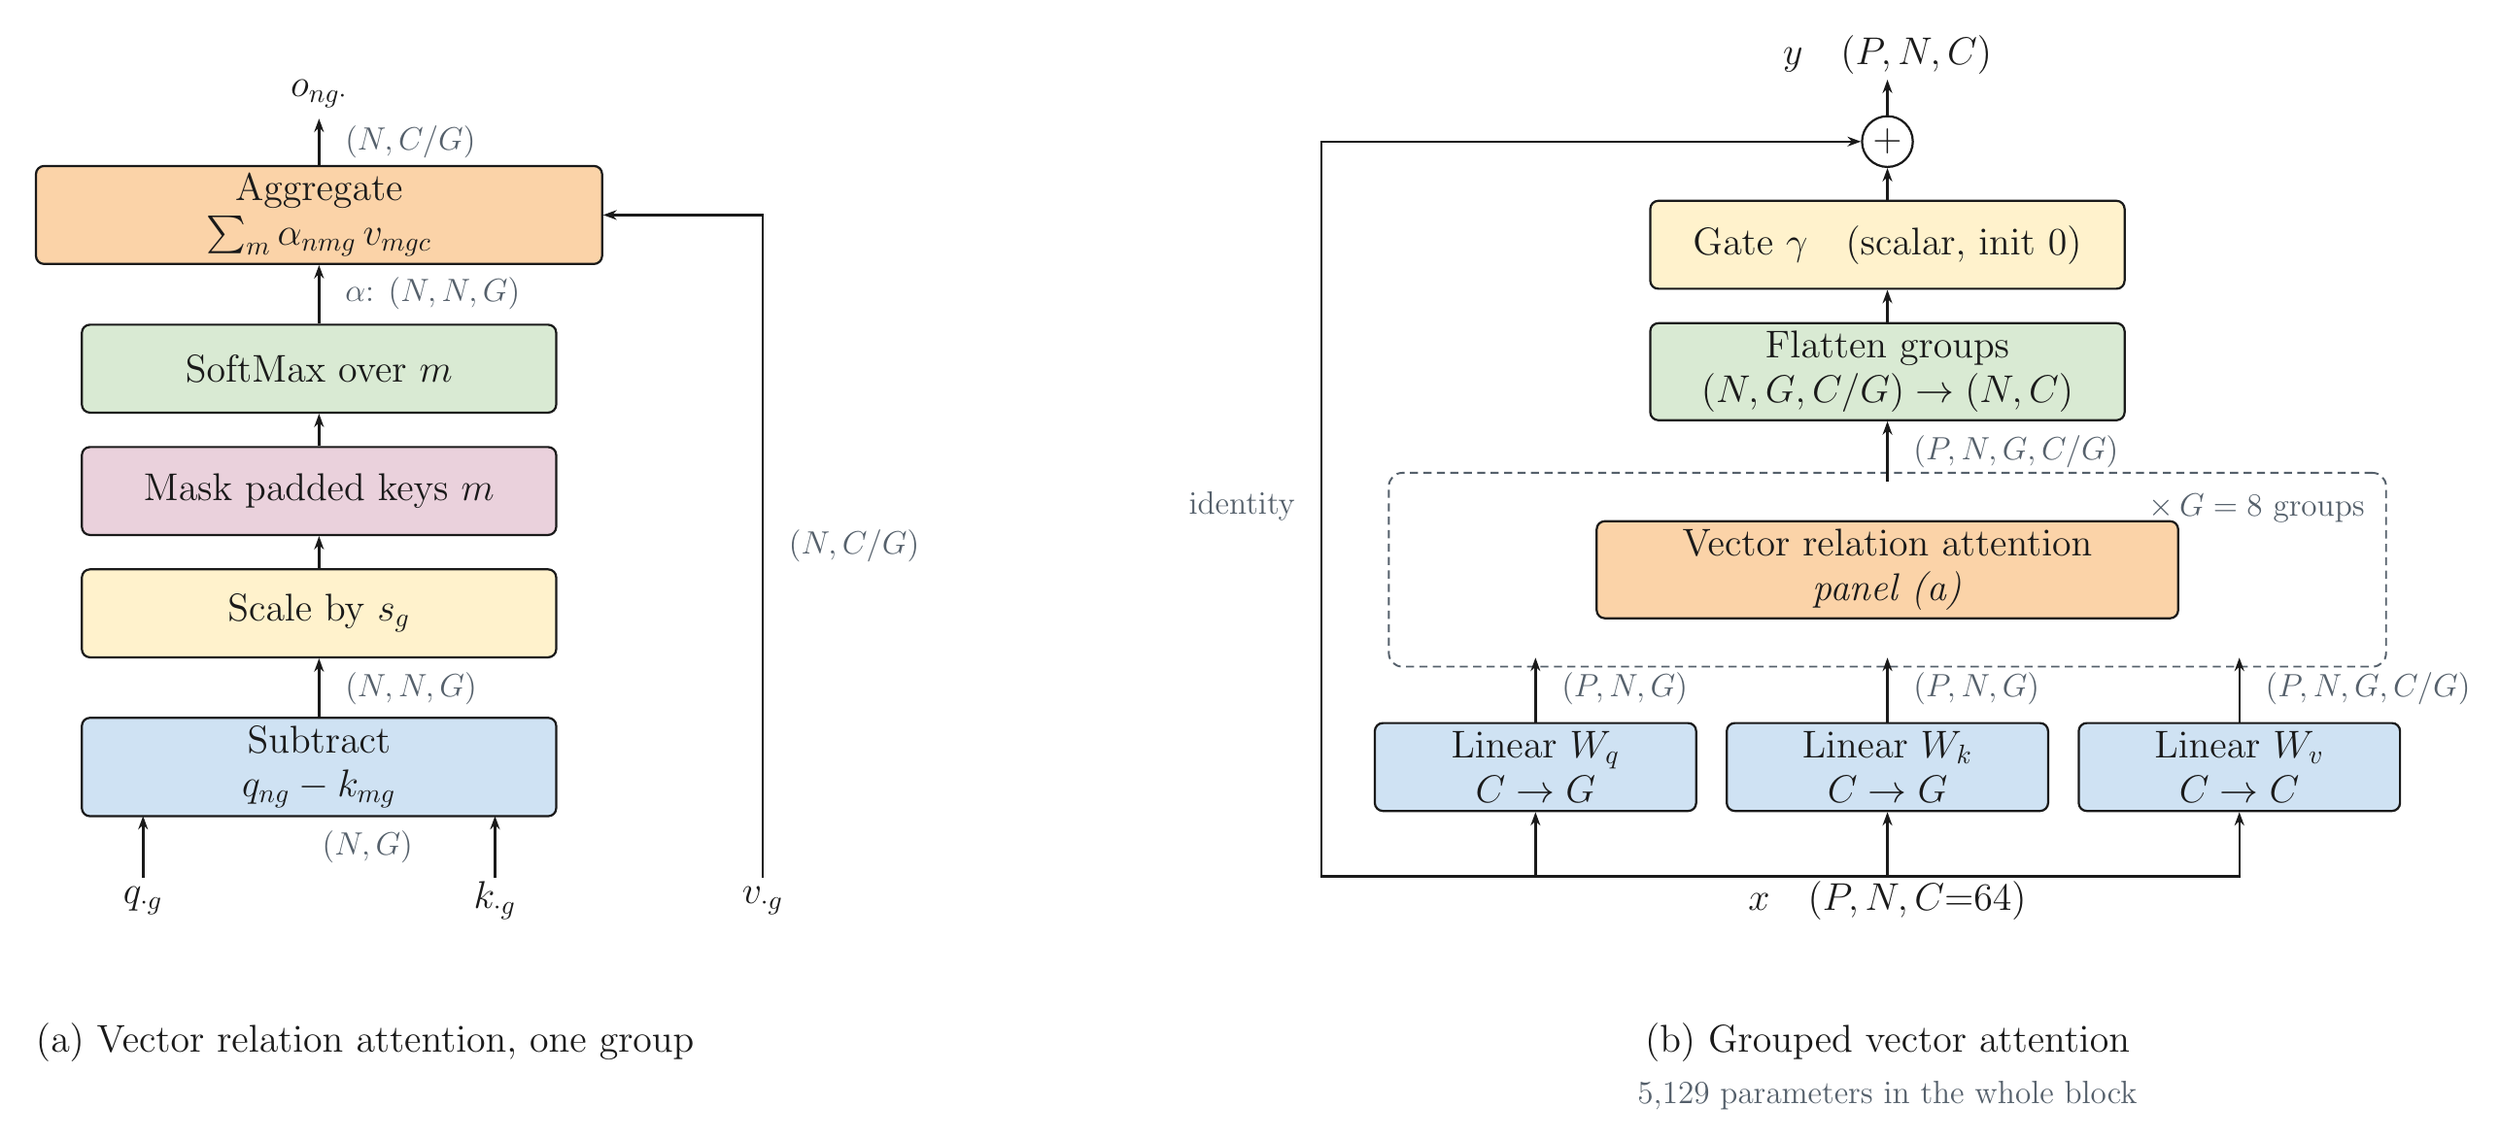
\begin{tikzpicture}[
    blk/.style  ={draw=bInk, line width=0.8pt, rounded corners=3pt, align=center,
                  minimum height=1.15cm, inner xsep=6pt, inner ysep=3pt,
                  text=bInk, font=\fontsize{14}{16.5}\selectfont},
    io/.style   ={align=center, text=bInk, font=\fontsize{14.5}{17}\selectfont},
    % inner sep 1pt so a shape label fits in the gap between two boxes
    shp/.style  ={align=center, text=bMuted, inner sep=1pt,
                  font=\fontsize{12}{14}\selectfont},
    ttl/.style  ={align=center, text=bInk, font=\fontsize{15}{17}\selectfont},
    flow/.style ={-{Stealth[length=5pt,width=3.6pt]}, draw=bInk, line width=0.9pt},
    aux/.style  ={-{Stealth[length=5pt,width=3.6pt]}, draw=bRed, line width=0.9pt,
                  dash pattern=on 3pt off 2pt},
    grp/.style  ={draw=bMuted, line width=0.7pt, dash pattern=on 3pt off 2pt,
                  rounded corners=5pt},
    op/.style   ={draw=bInk, line width=0.8pt, circle, inner sep=1.6pt, fill=white,
                  text=bInk, font=\fontsize{14}{14}\selectfont},
  ]
% ====== panel (a): vector relation attention ======
\node[io, anchor=center] at (-2.30,0.00) {$q_{\cdot g}$};
\node[io, anchor=center] at (2.30,0.00) {$k_{\cdot g}$};
\node[io, anchor=center] at (5.80,0.00) {$v_{\cdot g}$};
\node[blk, fill=bLin, minimum width=6.20cm] (sub) at (0.00,1.75) {Subtract\\$q_{ng}-k_{mg}$};
\node[blk, fill=bNorm, minimum width=6.20cm] (scl) at (0.00,3.76) {Scale by $s_g$};
\node[blk, fill=bMask, minimum width=6.20cm] (msk) at (0.00,5.36) {Mask padded keys $m$};
\node[blk, fill=bSoft, minimum width=6.20cm] (sfm) at (0.00,6.96) {SoftMax over $m$};
\node[blk, fill=bAgg, minimum width=7.40cm] (agg) at (0.00,8.97) {Aggregate\\$\sum_m \alpha_{nmg}\,v_{mgc}$};
\draw[flow] (-2.30,0.30) -- (-2.30,1.11);
\draw[flow] (2.30,0.30) -- (2.30,1.11);
\draw[flow] (sub) -- (scl);
\draw[flow] (scl) -- (msk);
\draw[flow] (msk) -- (sfm);
\draw[flow] (sfm) -- (agg);
\draw[flow] (5.80,0.30) -- (5.80,8.97) -- (agg.east);
\draw[flow] (agg.north) -- (0.00,10.23);
\node[io, anchor=center] at (0.00,10.55) {$o_{n g \cdot}$};
\node[shp, anchor=west] at (0.00,0.71) {$(N,G)$};
\node[shp, anchor=west] at (0.30,2.78) {$(N,N,G)$};
\node[shp, anchor=west] at (0.30,7.94) {$\alpha$: $(N,N,G)$};
\node[shp, anchor=west] at (0.30,9.92) {$(N,C/G)$};
\node[shp, anchor=west] at (6.10,4.64) {$(N,C/G)$};
\node[ttl, anchor=center] at (0.60,-1.85) {(a)~Vector relation attention, one group};
% ====== panel (b): grouped vector attention ======
\node[io, anchor=center] at (20.50,0.00) {$x$\quad$(P,N,C{=}64)$};
\node[blk, fill=bLin, minimum width=4.20cm] (wq) at (15.90,1.75) {Linear $W_q$\\$C\to G$};
\node[blk, fill=bLin, minimum width=4.20cm] (wk) at (20.50,1.75) {Linear $W_k$\\$C\to G$};
\node[blk, fill=bLin, minimum width=4.20cm] (wv) at (25.10,1.75) {Linear $W_v$\\$C\to C$};
\draw[flow] (20.50,0.32) -- (15.90,0.32) -- (wq.south);
\draw[flow] (20.50,0.32) -- (20.50,0.32) -- (wk.south);
\draw[flow] (20.50,0.32) -- (25.10,0.32) -- (wv.south);
\node[blk, fill=bAgg, minimum width=7.60cm] (vra) at (20.50,4.33) {Vector relation attention\\\emph{panel (a)}};
\node[grp, fit={(14.10,3.18) (26.90,5.48)}] (grp) {};
\node[shp, anchor=north east] at (26.78,5.36) {$\times\,G=8$ groups};
\draw[flow] (wq.north) -- (15.90,3.18);
\draw[flow] (wk.north) -- (20.50,3.18);
\draw[flow] (wv.north) -- (25.10,3.18);
\node[blk, fill=bSoft, minimum width=6.20cm] (flt) at (20.50,6.92) {Flatten groups\\$(N,G,C/G)\to(N,C)$};
\node[blk, fill=bNorm, minimum width=6.20cm] (gam) at (20.50,8.58) {Gate $\gamma$\quad(scalar, init $0$)};
\node[op] (add) at (20.50,9.93) {$+$};
\node[io, anchor=center] at (20.50,11.06) {$y$\quad$(P,N,C)$};
\draw[flow] (20.50,5.48) -- (flt.south);
\draw[flow] (flt) -- (gam);
\draw[flow] (gam.north) -- (add.south);
\draw[flow] (add.north) -- (20.50,10.74);
\draw[flow] (20.50,0.32) -- (13.10,0.32) -- (13.10,9.93) -- (add.west);
\node[shp, anchor=east] at (12.80,5.16) {identity};
\node[shp, anchor=west] at (16.20,2.78) {$(P,N,G)$};
\node[shp, anchor=west] at (20.80,2.78) {$(P,N,G)$};
\node[shp, anchor=west] at (25.40,2.78) {$(P,N,G,C/G)$};
\node[shp, anchor=west] at (20.80,5.88) {$(P,N,G,C/G)$};
\node[ttl, anchor=center] at (20.50,-1.85) {(b)~Grouped vector attention};
\node[shp, anchor=center] at (20.50,-2.55) {5{,}129 parameters in the whole block};

\end{tikzpicture}
\end{document}
